\documentclass{standalone}
\usepackage{tikz}
\usetikzlibrary{patterns, positioning}


\begin{document}
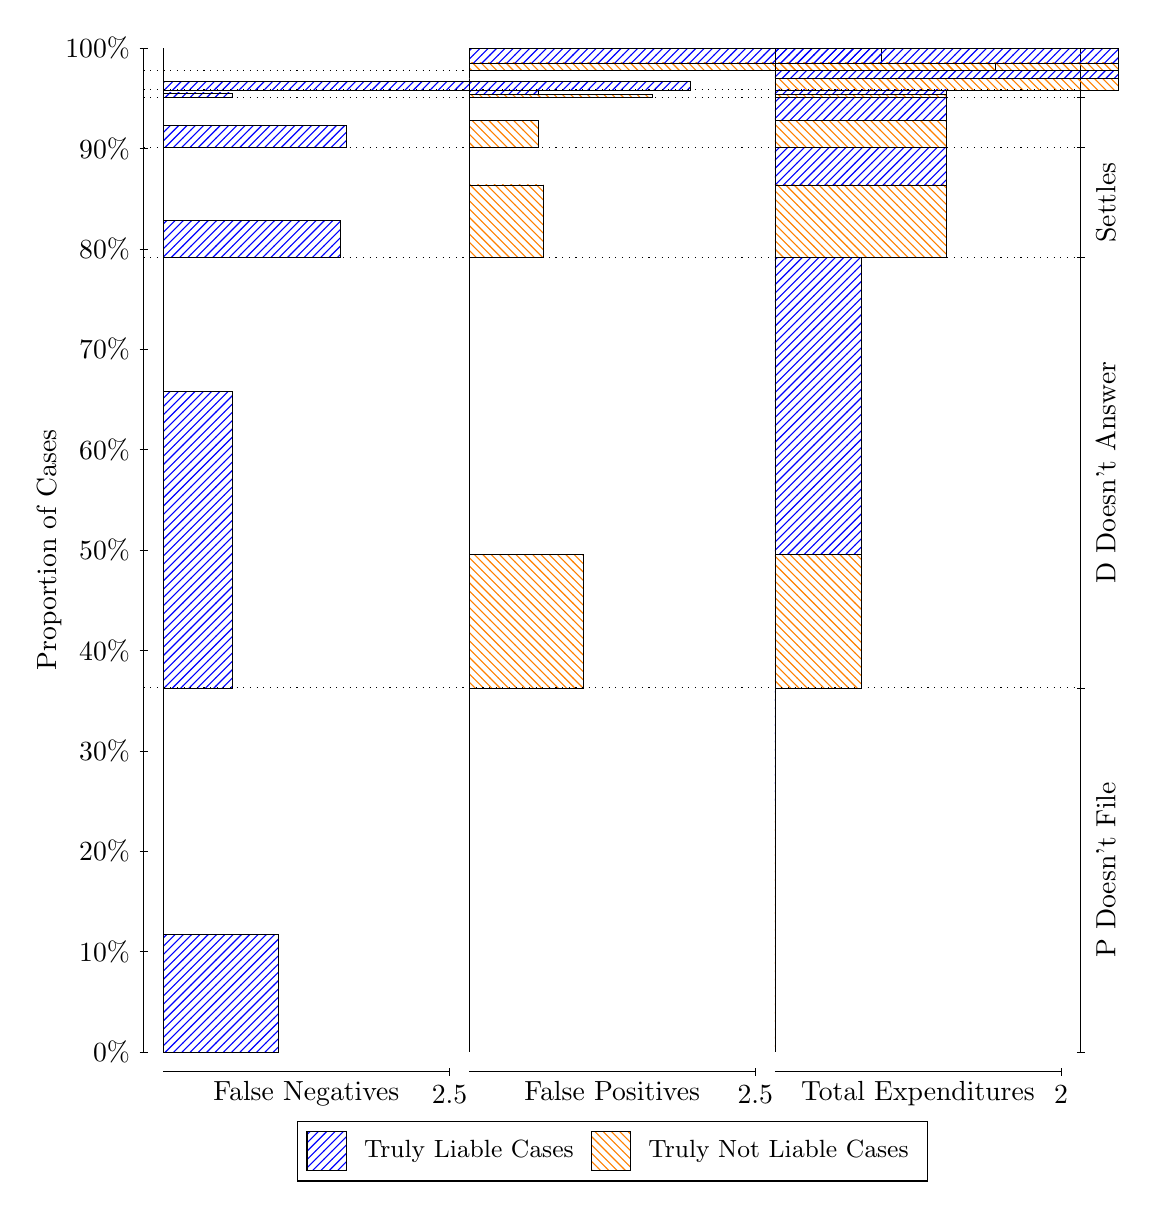
\begin{tikzpicture}
\draw[black, very thin] (1.5,1.75) -- (1.5,14.5);
\node[rotate=90, text=black, anchor=center] at (0.3, 8.125) {Proportion of Cases};
\draw[black, very thin] (1.45,1.75) -- (1.55,1.75);
\node[text=black, anchor=east] at (1.45, 1.75) {0\%};
\draw[black, very thin] (1.45,3.025) -- (1.55,3.025);
\node[text=black, anchor=east] at (1.45, 3.025) {10\%};
\draw[black, very thin] (1.45,4.3) -- (1.55,4.3);
\node[text=black, anchor=east] at (1.45, 4.3) {20\%};
\draw[black, very thin] (1.45,5.575) -- (1.55,5.575);
\node[text=black, anchor=east] at (1.45, 5.575) {30\%};
\draw[black, very thin] (1.45,6.85) -- (1.55,6.85);
\node[text=black, anchor=east] at (1.45, 6.85) {40\%};
\draw[black, very thin] (1.45,8.125) -- (1.55,8.125);
\node[text=black, anchor=east] at (1.45, 8.125) {50\%};
\draw[black, very thin] (1.45,9.4) -- (1.55,9.4);
\node[text=black, anchor=east] at (1.45, 9.4) {60\%};
\draw[black, very thin] (1.45,10.675) -- (1.55,10.675);
\node[text=black, anchor=east] at (1.45, 10.675) {70\%};
\draw[black, very thin] (1.45,11.95) -- (1.55,11.95);
\node[text=black, anchor=east] at (1.45, 11.95) {80\%};
\draw[black, very thin] (1.45,13.225) -- (1.55,13.225);
\node[text=black, anchor=east] at (1.45, 13.225) {90\%};
\draw[black, very thin] (1.45,14.5) -- (1.55,14.5);
\node[text=black, anchor=east] at (1.45, 14.5) {100\%};

\draw[black, very thin] (13.4,1.75) -- (13.4,14.5);
\draw[black, very thin] (13.35,1.75) -- (13.45,1.75);
\node[anchor=west] at (13.35, 1.75) {};
\draw[black, very thin] (13.35,6.3743) -- (13.45,6.3743);
\node[anchor=west] at (13.35, 6.3743) {};
\draw[black, very thin] (13.35,11.839) -- (13.45,11.839);
\node[anchor=west] at (13.35, 11.839) {};
\draw[black, very thin] (13.35,13.236) -- (13.45,13.236);
\node[anchor=west] at (13.35, 13.236) {};
\draw[black, very thin] (13.35,13.869) -- (13.45,13.869);
\node[anchor=west] at (13.35, 13.869) {};
\draw[black, very thin] (13.35,13.969) -- (13.45,13.969);
\node[anchor=west] at (13.35, 13.969) {};
\draw[black, very thin] (13.35,14.218) -- (13.45,14.218);
\node[anchor=west] at (13.35, 14.218) {};
\draw[black, very thin] (13.35,14.5) -- (13.45,14.5);
\node[anchor=west] at (13.35, 14.5) {};

\draw[black, very thin, pattern color=blue, pattern=north east lines] (1.75,1.75) rectangle (3.2033,3.2409);
\draw[black, very thin, pattern color=orange, pattern=north west lines] (1.75,3.2409) rectangle (1.75,6.3743);
\draw[black, very thin, pattern color=blue, pattern=north east lines] (1.75,6.3743) rectangle (2.622,10.141);
\draw[black, very thin, pattern color=orange, pattern=north west lines] (1.75,10.141) rectangle (1.75,11.839);
\draw[black, very thin, pattern color=blue, pattern=north east lines] (1.75,11.839) rectangle (4.0027,12.313);
\draw[black, very thin, pattern color=orange, pattern=north west lines] (1.75,12.313) rectangle (1.75,13.236);
\draw[black, very thin, pattern color=blue, pattern=north east lines] (1.75,13.236) rectangle (4.0753,13.521);
\draw[black, very thin, pattern color=orange, pattern=north west lines] (1.75,13.521) rectangle (1.75,13.869);
\draw[black, very thin, pattern color=blue, pattern=north east lines] (1.75,13.869) rectangle (2.622,13.929);
\draw[black, very thin, pattern color=orange, pattern=north west lines] (1.75,13.929) rectangle (1.75,13.969);
\draw[black, very thin, pattern color=blue, pattern=north east lines] (1.75,13.969) rectangle (8.4353,14.076);
\draw[black, very thin, pattern color=orange, pattern=north west lines] (1.75,14.076) rectangle (1.75,14.218);
\draw[black, very thin, pattern color=orange, pattern=north west lines] (1.75,14.218) rectangle (1.75,14.31);
\draw[black, very thin, pattern color=blue, pattern=north east lines] (1.75,14.31) rectangle (1.75,14.5);
\draw[black, very thin, pattern color=orange, pattern=north west lines] (5.6333,1.75) rectangle (5.6333,4.8835);
\draw[black, very thin, pattern color=blue, pattern=north east lines] (5.6333,4.8835) rectangle (5.6333,6.3743);
\draw[black, very thin, pattern color=orange, pattern=north west lines] (5.6333,6.3743) rectangle (7.0867,8.0719);
\draw[black, very thin, pattern color=blue, pattern=north east lines] (5.6333,8.0719) rectangle (5.6333,11.839);
\draw[black, very thin, pattern color=orange, pattern=north west lines] (5.6333,11.839) rectangle (6.578,12.762);
\draw[black, very thin, pattern color=blue, pattern=north east lines] (5.6333,12.762) rectangle (5.6333,13.236);
\draw[black, very thin, pattern color=orange, pattern=north west lines] (5.6333,13.236) rectangle (6.5053,13.583);
\draw[black, very thin, pattern color=blue, pattern=north east lines] (5.6333,13.583) rectangle (5.6333,13.869);
\draw[black, very thin, pattern color=orange, pattern=north west lines] (5.6333,13.869) rectangle (7.9587,13.908);
\draw[black, very thin, pattern color=blue, pattern=north east lines] (5.6333,13.908) rectangle (6.5053,13.969);
\draw[black, very thin, pattern color=orange, pattern=north west lines] (5.6333,13.969) rectangle (5.6333,14.112);
\draw[black, very thin, pattern color=blue, pattern=north east lines] (5.6333,14.112) rectangle (5.6333,14.218);
\draw[black, very thin, pattern color=orange, pattern=north west lines] (5.6333,14.218) rectangle (12.319,14.31);
\draw[black, very thin, pattern color=blue, pattern=north east lines] (5.6333,14.31) rectangle (10.865,14.5);
\draw[black, very thin, pattern color=orange, pattern=north west lines] (9.5167,1.75) rectangle (9.5167,4.8835);
\draw[black, very thin, pattern color=blue, pattern=north east lines] (9.5167,4.8835) rectangle (9.5167,6.3743);
\draw[black, very thin, pattern color=orange, pattern=north west lines] (9.5167,6.3743) rectangle (10.607,8.0719);
\draw[black, very thin, pattern color=blue, pattern=north east lines] (9.5167,8.0719) rectangle (10.607,11.839);
\draw[black, very thin, pattern color=orange, pattern=north west lines] (9.5167,11.839) rectangle (11.697,12.762);
\draw[black, very thin, pattern color=blue, pattern=north east lines] (9.5167,12.762) rectangle (11.697,13.236);
\draw[black, very thin, pattern color=orange, pattern=north west lines] (9.5167,13.236) rectangle (11.697,13.583);
\draw[black, very thin, pattern color=blue, pattern=north east lines] (9.5167,13.583) rectangle (11.697,13.869);
\draw[black, very thin, pattern color=orange, pattern=north west lines] (9.5167,13.869) rectangle (11.697,13.908);
\draw[black, very thin, pattern color=blue, pattern=north east lines] (9.5167,13.908) rectangle (11.697,13.969);
\draw[black, very thin, pattern color=orange, pattern=north west lines] (9.5167,13.969) rectangle (13.877,14.112);
\draw[black, very thin, pattern color=blue, pattern=north east lines] (9.5167,14.112) rectangle (13.877,14.218);
\draw[black, very thin, pattern color=orange, pattern=north west lines] (9.5167,14.218) rectangle (13.877,14.31);
\draw[black, very thin, pattern color=blue, pattern=north east lines] (9.5167,14.31) rectangle (13.877,14.5);
\draw[black, dotted] (1.5,6.3743) -- (13.4,6.3743);
\draw[black, dotted] (1.5,11.839) -- (13.4,11.839);
\draw[black, dotted] (1.5,13.236) -- (13.4,13.236);
\draw[black, dotted] (1.5,13.869) -- (13.4,13.869);
\draw[black, dotted] (1.5,13.969) -- (13.4,13.969);
\draw[black, dotted] (1.5,14.218) -- (13.4,14.218);
\draw[black, very thin] (1.75,1.5) -- (5.3833,1.5);
\node[text=black, anchor=north] at (3.5667, 1.5) {False Negatives};
\draw[black, very thin] (5.3833,1.45) -- (5.3833,1.55);
\node[text=black, anchor=north] at (5.3833, 1.45) {2.5};

\draw[black, very thin] (5.6333,1.5) -- (9.2667,1.5);
\node[text=black, anchor=north] at (7.45, 1.5) {False Positives};
\draw[black, very thin] (9.2667,1.45) -- (9.2667,1.55);
\node[text=black, anchor=north] at (9.2667, 1.45) {2.5};

\draw[black, very thin] (9.5167,1.5) -- (13.15,1.5);
\node[text=black, anchor=north] at (11.333, 1.5) {Total Expenditures};
\draw[black, very thin] (13.15,1.45) -- (13.15,1.55);
\node[text=black, anchor=north] at (13.15, 1.45) {2};

\node[text=black, centered, rotate=90] at (13.72, 4.0622) {P Doesn't File};
\node[text=black, centered, rotate=90] at (13.72, 9.1065) {D Doesn't Answer};
\node[text=black, centered, rotate=90] at (13.72, 12.537) {Settles};





\draw (7.449999999999999,1.5) node[draw=none] (baseCoordinate) {};
\begin{scope}[align=center]
        \matrix[scale=0.5, draw=black, below=0.5cm of baseCoordinate, nodes={draw}, column sep=0.1cm]{
            \node[rectangle, draw, minimum width=0.5cm, minimum height=0.5cm, pattern color=blue, pattern=north east lines] {}; &
            \node[draw=none, font=\small, text=black] (B) {Truly Liable Cases}; &
            \node[rectangle, draw, minimum width=0.5cm, minimum height=0.5cm, pattern color=orange, pattern=north west lines] {}; &
            \node[draw=none, font=\small, text=black] (B) {Truly Not Liable Cases}; \\
            };
\end{scope}

\end{tikzpicture}
\end{document}